% !TeX root = ../DistributedConsensus.tex
\chapter{Previous Approaches to solving the Problem}
\label{chap:previous-attempts}
	% TODO: Recursive "Produce", reachability, validation issues.	
	Previous attempts at producing the order of execution have been made, each with shortcomings, that have led to the development of the implemented solution.
	
	\newpar These attempts and their shortcomings are detailed below.
	
	\section{Recursive Traversal of the Distributed Graph}
	Assume that it is desired that any given event in a distributed DCR graph is able to initiate a gathering and production of an order of execution, in cooperation with reachable events in the graph. 
	
	\subsection{Analysis}
	If each event only knows a subset of the other events of a workflow, then simply merging the histories of that subset of neighbours will not create a complete history of what has happened up until that moment in time. 
	
	Because of these problems an algorithm which is able to gather information from the entire workflow without knowing all the nodes is developed. Such an algorithm needs to be measured in its ability to reach all reachable events in the graph, as well as its ability to handle relation cycles. 
	
	\subsection{The Produce Algorithm}
	Given a DCR graph where all events are not reachable from the starting event, the algorithm should fetch and merge the histories of each event in the graph into one history.
	
	This is accomplished by recursively contacting neighbouring events and asking them for their history while stitching the neighbours' history with its own history. To handle cycles, the use of a trace of previously contacted events is send from each event to the next.
	
	\newpar The implementation uses two lists, called \texttt{request trace} and \texttt{wait for}.
	The algorithm propagates throughout the graph using recursion with checks during execution in order to avoid infinite cycles of requests. 
	
	When an event receives a request for its history, it adds every reachable event from itself to \texttt{wait for}. Then the event crosschecks the event IDs of the \texttt{request trace} and the event's own \texttt{wait for} list. Any event ID in \texttt{wait for} that exists in \texttt{request trace} is removed and the history of the event is returned to the requester. Any remaining events in \texttt{wait for} gets sent requests for history their history with the ID of the event appended to the \texttt{request trace}. 
	
	\subsection{Implementation}
	\begin{algorithmic}
		\State Event receives request for history with a \texttt{request trace}, $T$.
		\State Event has internal \texttt{wait for}, $W$
		\State
		\State $W\gets W::$ reachable events \Comment Add all reachable events to \texttt{wait for}.
		\If {$W=\emptyset$}
			\Return own history
		\Else
			\State $W\gets W-T$ \Comment Remove every event in $T$ from $W$. Cycles avoided.
			\State $T\gets T::ownID$ \Comment Append own event ID to $T$.
			\State
			\ForAll {$w$ in $W$} 
				\State request history from $w$ with $T$ \Comment Request from neighbours with new \texttt{trace}.
			\EndFor
			\State wait for receiving histories
			\State stitch received histories with own history
			\State
			\Return stitched histories
		\EndIf
	\end{algorithmic}
	
	\newpar This algorithm is in fact a modified version of the flooding search algorithm for searching in unstructured peer to peer networks. In produce each node visited returns something and not only the searched for node. Furthermore the flooding algorithm is often implemented with a time limit on the search and therefore does not care about cycles, which is handled more effeciently in the produce algorithm.
	
	\subsection{Correctness}
	Since this algorithm is a modfied version of the flooding algorithm it has most of the same traits with respect to reachability of the algorithm. If there exits a path from the beginning node to all other nodes in the workflow, the algorithm is. 
	
	\subsection{Performance}
	This algorithm has a worst case message performance of O(2*N$^2$) where N is the number of events in the system. This occurs when the graph is fully connected, and all events therefore have relations to all other events in the graph. 
	
	Realistically this situation will rarely occur since DCR graphs. \todo{Since wat?}
	
	\newpar Caching history produced of an event before transferring it to a requesting event could improve performance, but presents new problems. 
	
	Certain issues arise if an event with neighbours is the last event in what would have been a produce cycle and due to tracing returns its own local history which would then be cached. This event would then never return the histories of its neighbours if contacted again from a different event, but would instead only return its own history due to caching. 
	
	The neighbours history of the neighbours would then only be produced once, and therefore pass through a single, possibly malicious, node. The lack of redundancy in the system therefore presents an issue when validating histories.
	
	It is therefore necessary to produce redundant histories, which makes caching impossible.
	
	\subsection{Issues with Recursive Traversal of the Distributed Graph}
	\todo[inline]{Omformulér afsnit om, at det er tæt på umuligt at validere historik (specielt vha. DCR-regler) uden at kende hele workflowet.}
	
	There is a couple of pitfalls with the algorithm. If malicious events are introduced in the DCR graph, the same problems arise as with the graph where the beginning node had relations with the rest of the graph. 
	
	\newpar That is, if the neighbouring nodes do not know enough of each other, there is no way of making sure that the returned history is correct. Furthermore, this uncertainty is amplified due to the fact that for each contacted event with lacking information, it is possible to tamper with the history of the recursively called events, or even add history of non existent events. Therefore some action must be taken to handle these pitfalls. \todo{Wat.}
	
	\section{Use of the Transitive Closure in Order to Gain Extra Information}
	It is desired to be able to guarantee that the order of execution is as correct as the information provided by events allow it to be. Increasing reachability of actions in the history will provide more information about the actions that have occurred, even if these actions have no existing relation. 
	
	Since a strict partial order is a directed acyclic graph, the transitive closure of the graph can be found, to find more happens-before relations. This is useful when determining what actions are part of an execution. 
	
	Finding the transitive closure does not always give better results, and the \texttt{Collapse} solution was found instead. 
	In \autoref{fig:problem:trans} the result of finding the transitive closure on the joined histories of two events is shown. 
	Compare the result to the result of using the collapse approach in \autoref{fig:problem:collapse}. 
	The actions marked with a grey color are concurrent after the transitive closure has been found, but actually happen in order, which is seen when using the collapse approach. 
	
	\subsection{Complexity}
	We implemented the finding of the transitive closure as a depth first search, which has a running time of $\mathcal{O}(V + E)$. \textit{Collapse} is therefore a more efficient as well as a more precise way of finding an order of execution as described in \autoref{chap:order-of-execution}.
	
	
	\begin{figure}
		\centering
		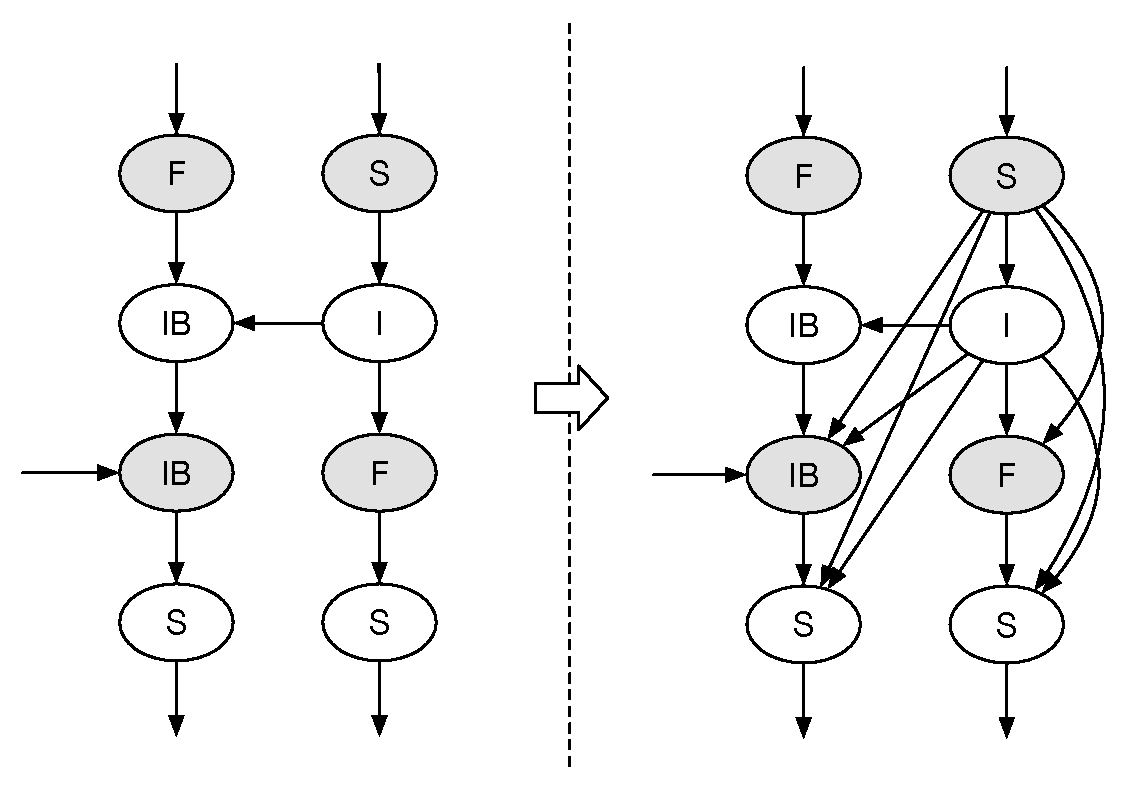
\includegraphics[width=\textwidth]{8problem/images/trans.pdf}
		\caption{The result of finding the transitive closure on from the actions of an event. Note that the grey \texttt{ExecuteFinish}, \texttt{IncludedBy} and\texttt{ExecuteStart} seem to happen concurrently.}
		\label{fig:problem:trans}
	\end{figure}
	
	\begin{figure}
		\centering
		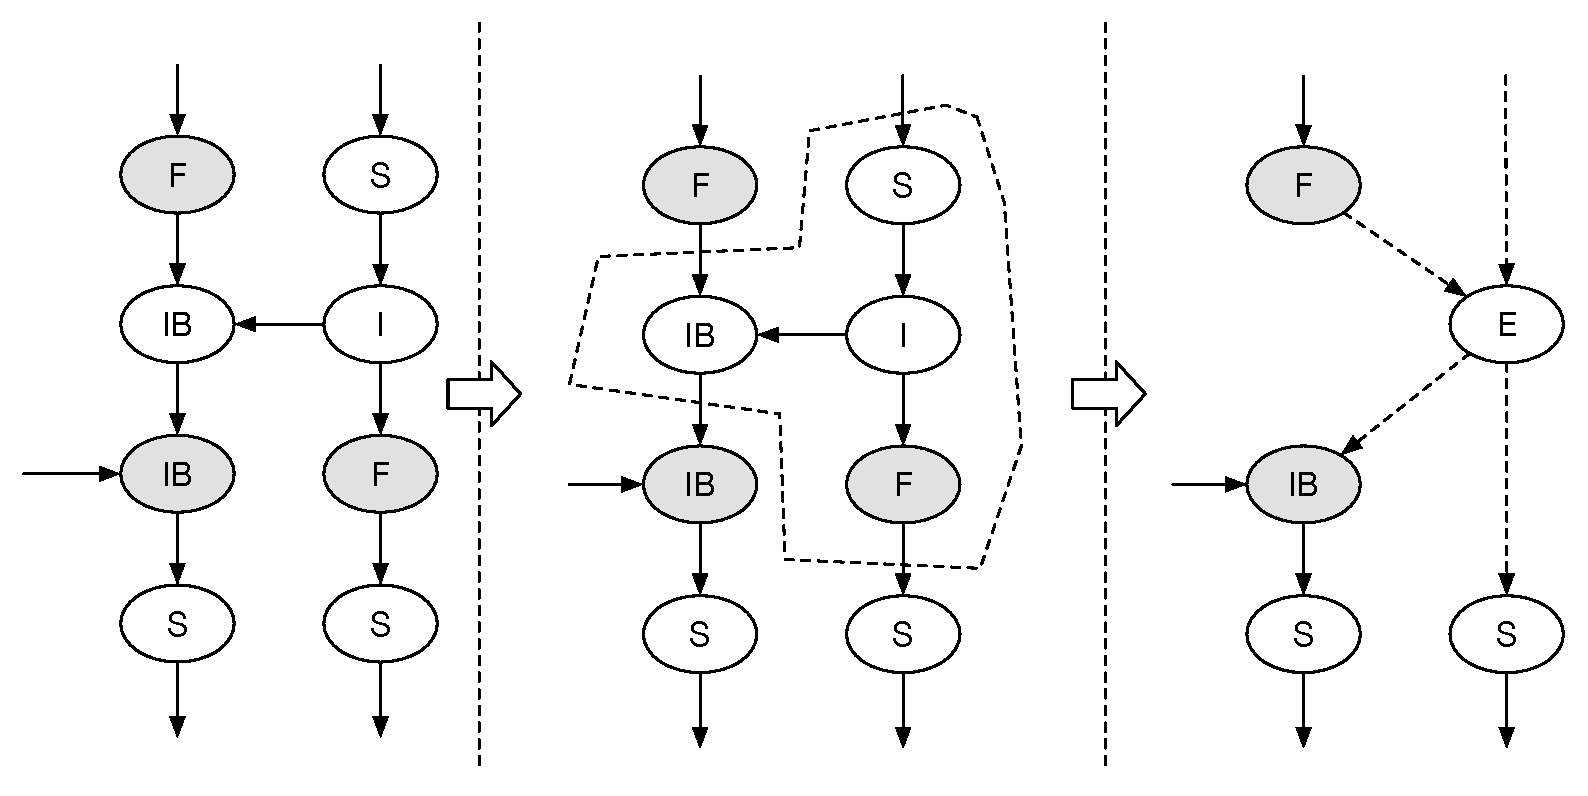
\includegraphics[width=\textwidth]{8problem/images/collapse.pdf}
		\caption{The result of finding an execution using \textit{Collapse}. Note that the grey  \texttt{ExecuteFinish} happens before the next execution and that the \texttt{IncludedBy} action happens after the execution.}
		\label{fig:problem:collapse}
	\end{figure}
	
	%\begin{figure}
	%	\centering
	%	\def\svgwidth{0.42\columnwidth}
	%	\fontsize{6}{8}\selectfont
	%	\import{5connect/images/}{3executionswithtransitive.pdf_tex}
	%	\caption{3 executions before and after applying execution transitive closure.}
	%	\label{fig:connect:3executionstrans}
	%\end{figure}
	
	%\begin{algorithm}
	%	\begin{algorithmic}
	%	\Function{Execution Transitive-Closure}{history}
	%		\State startFromSet $\leftarrow$ actions with no incomming edges in history
	%		\ForAll{fromAction in startFromSet}
	%			\State neighbourActions $\leftarrow$ \Call{GetNeighboursOfNeighbours}{fromAction}
	%			\ForAll{neighbour in neighbourActions}
	%				\If {neighbour is execution}
	%					\State history $\leftarrow$ \Call{addEdge}{fromAction, neighbour, history}
	%					\State startFromSet $\leftarrow$ \Call{add}{neighbour, startFromSet}
	%				\Else
	%					\State neighbourActions $\leftarrow$ \Call{Union}{neighbour.neighbours, neighbourActions}
	%				\EndIf
	%			\EndFor
	%		\EndFor
	%		\State 
	%		\Return graph
	%	\EndFunction
	%	\end{algorithmic}
	%	\caption{Transitive Closure Algorithm}
	%\end{algorithm}
	
	